\chapter{Théorèmes de géométrie et de trigonométrie}\label{a.trig}


%%%%%%%%%%%%%%%%%%%%%%%%%%%%%%%%%%%%%%%%%%%%%%%%%%%%%%%%%%%%%%%

Cette annexe présente des théorèmes de géométrie et de trigonométrie qui peuvent ne pas être familiers au lecteur, ainsi que des théorèmes qui peuvent être familiers mais dont les démonstrations ne le sont pas. La section~\ref{a.triangles} présente trois formules pour calculer l'aire d'un triangle. La section~\ref{a.trig-identities} démontre des formules trigonométriques. Bien que les formules soient pour la plupart familières, les étudiants les apprennent souvent par cœur ou les consultent sans jamais en voir la démonstration. Les sections suivantes contiennent les démonstrations de théorèmes plus avancés en géométrie :  le théorème de la bissectrice dans la section~\ref{a.bisector}, le théorème de Ptolémée qui relie les côtés et les diagonales d'un quadrilatère circonscrit à un cercle dans  la  section~\ref{a.ptolemy}, le théorème de Ceva dans la  section~\ref{a.ceva} et le théorème de Ménélaüs  dans la section~\ref{a.menelaus}.

%%%%%%%%%%%%%%%%%%%%%%%%%%%%%%%%%%%%%%%%%%%%%%%%%%%%%%%%%%%

\section{Théorèmes sur les triangles}\label{a.triangles}

%%%%%%%%%%%%%%%%%%%%%%%%%%%%%%%%%%%%%%%%%%%%%%%%%%%%%%%%%%%

\subsection{Calcul de l'aire d'un triangle}


La formule standard pour calculer l'aire d'un triangle à partir de la base et de la hauteur est bien connue. Elle peut être démontrée à l'aide de diverses méthodes géométriques.

\begin{theorem} L'aire du triangle $\triangle ABC$ est donnée par 
\begin{align}
\triangle ABC=\frac{1}{2}bh\,,\label{eq.area-from-base}
\end{align}
où la base $b$ est l'un des côtés du triangle  et la hauteur $h$ est la distance de $b$ au sommet opposé (fig.~\ref{f.area-base-height-1}).
\end{theorem}

\begin{proof}
La figure~\ref{f.area-base-height-2} montre qu'en \og coupant\fg{} le triangle à la moitié de sa hauteur, on peut \og déplacer\fg{} les triangles ombrés pour former un rectangle de même surface que le triangle. La base du rectangle est $b$ et sa hauteur est $h/2$.
\end{proof}



\vspace{0.4cm}

\begin{minipage}{0.4\textwidth}
\centering    
\begin{tikzpicture}[scale=.55]
\coordinate (A) at (0,0);
\coordinate (C) at (7,0);
\path[name path=ab] (A) -- +(60:5.5);
\path[name path=cb] (C) -- +(140:7);
\path[name intersections={of=ab and cb,by={B}}];
\draw (A) -- node[below] {$b$} (C) -- node[above] {$a$} (B) -- node[above,xshift=-2pt] {$c$}  cycle;
\node[left] at (A) {$A$};
\node[above right,xshift=4pt] at (A) {$\theta$};
\node[above] at (B) {$B$};
\node[right] at (C) {$C$};
\draw (B) -- node[right,yshift=-12pt] {$h=c\sin\theta$} 
  (B|-A) coordinate (H);
\draw[rotate=90] (H) rectangle +(8pt,8pt);
\end{tikzpicture}
%\includegraphics[width=\textwidth]{FigA1a}
         \captionof{figure}{Calcul de l'aire d'un triangle à partir de la base et de la hauteur.}\label{f.area-base-height-1}
         
     \end{minipage}
     \hspace{3em}
     \begin{minipage}{0.4\textwidth}
\centering         
\begin{tikzpicture}[scale=.55]
\coordinate (A) at (0,0);
\coordinate (C) at (7,0);
\path[name path=ab] (A) -- +(60:5.5);
\path[name path=cb] (C) -- +(140:7);
\path[name intersections={of=ab and cb,by={B}}];
\node[left] at (A) {$A$};
\node[above] at (B) {$B$};
\node[right] at (C) {$C$};
\path (B) -- node[right,near end] {$h/2$} (B|-A) coordinate (H);
\draw[rotate=90] (H) rectangle +(8pt,8pt);
\coordinate (K) at ($(H)!.5!(B)$);
\draw (A) -- node[below] {$b$} (C);
\draw (H) -- (K);
\coordinate (KA) at (K -| A);
\coordinate (KAB) at ($(A)!.5!(B)$);
\fill[color=white!50!red] (A) -- (KA) -- (KAB) -- cycle;
\fill[color=white!50!red] (B) -- (KAB) -- (K) -- cycle;
\coordinate (KC) at (K -| C);
\coordinate (KBC) at ($(B)!.5!(C)$);
\fill[color=white!50!blue] (C) -- (KC) -- (KBC) -- cycle;
\fill[color=white!50!blue] (B) -- (KBC) -- (K) -- cycle;
\draw[very thick,dashed] (A) -- (K -| A) -- (K -| C) -- (C);
\draw[very thick,dashed] (A) -- (B) -- (K);
\draw[very thick,dashed] (B) -- (C);
\path (K) -- node[inner sep=1pt, fill=white,right,
                 xshift=2pt,yshift=-3pt] {$h/2$} (B);
\end{tikzpicture}
%\includegraphics[width=\textwidth]{FigA1b}
         \captionof{figure}{Calcul de l'aire d'un triangle à partir de la base et de la hauteur.}\label{f.area-base-height-2}
     \end{minipage}

\vspace{0.4cm}




\begin{theorem} L'aire du triangle $\triangle ABC$ est donnée par 
\begin{align}\label{eq.area-from-sine}
\triangle ABC = \frac{1}{2}bc\sin \theta\,.
\end{align}
\end{theorem}
\begin{proof} Cela résulte du  théorème~\ref{eq.area-from-base} en utilisant 
$h=c\sin \theta$.
\end{proof}

%%%%%%%%%%%%%%%%%%%%%%%%%%%%%%%%%%%%%%%%%%%%%%%%%%%%%%%%%%%



\begin{theorem}[Héron] L'aire du triangle $\triangle ABC$ est donnée par \label{thm.heron} 
\[
\triangle ABC = \sqrt{s(s-a)(s-b)(s-c)}\,,
\]
où  le demi-périmètre $s$ du triangle est égal à $\frac{1}{2}(a+b+c)$.
\end{theorem}

\begin{proof}
Le rayon d'un cercle et une tangente qui coupe le rayon sont perpendiculaires. De plus, les longueurs des deux segments  tangents au cercle qui partent d'un même point sont égales. Par conséquent  (fig.~\ref{f.inscribed}),\footnote{Cela montre que le centre du cercle inscrit est l'intersection des trois bissectrices.}
\[
\triangle AOB'\cong \triangle AOC',\quad
\triangle BOA'\cong\triangle BOC',\quad
\triangle COA'\cong \triangle COB'\,.
\]
\begin{figure}[ht]
\centering
   \begin{tikzpicture}[scale=1.5]
% Draw base and path two lines at known angles
\draw (0,0) coordinate (a) node[xshift=-6pt] {$A$} -- (0:6) coordinate (b) node[xshift=6pt] {$B$};
\path[name path=ac] (a) -- +(50:4);
\path[name path=bc] (b) -- +(150:5);
% Get their intersection and draw lines between vertices
\path[name intersections={of=ac and bc,by=c}];
\node[above] at (c) {$C$};
\draw (a) -- (c) -- (b) -- (a);
% Label angles with tick marks
\draw (a) ++(0:4mm) arc (0:50:4mm);
\draw (a) ++(10:3.5mm) -- +(10:1mm);
\draw (a) ++(15:3.5mm) -- +(15:1mm);
\draw (a) ++(35:3.5mm) -- +(35:1mm);
\draw (a) ++(40:3.5mm) -- +(45:1mm);
\draw (b) ++(150:5mm) arc (150:180:5mm);
\draw (b) ++(157.5:4.5mm) -- +(157.5:1mm);
\draw (b) ++(172.5:4.5mm) -- +(172.5:1mm);
\draw (c) ++(230:3mm) arc (230:330:3mm);
\draw (c) ++(250:2.4mm) -- +(250:.9mm);
\draw (c) ++(255:2.4mm) -- +(255:.9mm);
\draw (c) ++(260:2.4mm) -- +(260:.9mm);
\draw (c) ++(300:2.4mm) -- +(300:.9mm);
\draw (c) ++(305:2.4mm) -- +(305:.9mm);
\draw (c) ++(310:2.4mm) -- +(310:.9mm);
% Path bisectors of two lines
\path[name path=bia] (a) -- +(25:3.5);
\path[name path=bib] (b) -- +(165:5);
% Intersection of angle bisectors
\path [name intersections={of=bia and bib,by=center}];
% Draw angle bisectors to center
\draw (a) -- (center);
\draw (c) -- (center);
\draw (b) -- (center);
% Draw radii
\draw (center) -- node[left] {$r$} ($(a)!(center)!(b)$) node[below,yshift=-2pt] {$C'$} coordinate (ap);
\draw (center) -- node[left,yshift=-4pt] {$r$} ($(a)!(center)!(c)$) node[above left] {$B'$} coordinate (bp);
\draw (center) -- node[right] {$r$} ($(b)!(center)!(c)$) node[above right] {$A'$} coordinate (cp);
% Draw dots
\vertex{center};
\node[above,xshift=3pt,yshift=7pt] at (center) {$O$};
% Draw right angle squares
\draw (ap) -- ++(90:4pt) -- ++(0:4pt) -- ++(-90:4pt);
\draw (bp) -- ++(-40:4pt) -- ++(-130:4pt) -- ++(-220:4pt);
\draw (cp) -- ++(-30:4pt) -- ++(-120:4pt) -- ++(-210:4pt);
% Labels of angles
\node[above,xshift=5pt,yshift=18pt] at (center) {$\gamma/2$};
\node[above left,xshift=-4pt,yshift=18pt] at (center) {$\gamma/2$};
\node[above right,xshift=3pt,yshift=-3pt] at (center) {$\beta/2$};
\node[below right,yshift=-3pt] at (center) {$\beta/2$};
\node[left,xshift=-5pt,yshift=2pt] at (center) {$\alpha/2$};
\node[below left,xshift=2pt,yshift=-4pt] at (center) {$\alpha/2$};
% Labels of line segments (names of points are weird...)
\path (a) -- node[below,yshift=-2pt] {$u$} (ap);
\path (a) -- node[left, xshift=-2pt] {$u$} (bp);
\path (b) -- node[above,yshift=2pt]  {$v$} (cp);
\path (b) -- node[below,xshift=-2pt] {$v$} (ap);
\path (c) -- node[above,xshift=-2pt] {$w$} (bp);
\path (c) -- node[above,xshift=2pt]  {$w$} (cp);
% Labels of sides
\draw[<->] ($(a)+(0,-10pt)$) -- node[fill=white] {$c$} 
           ($(b)+(0,-10pt)$);
\draw[<->] ($(a)+(-10pt,8pt)$) -- node[fill=white] {$b$}
           ($(c)+(-10pt,8pt)$);
\draw[<->] ($(b)+(6pt,10pt)$) -- node[fill=white] {$a$}
           ($(c)+(6pt,10pt)$);
% Inscribed circle
\node[very thick,dotted,draw,circle through=(ap)] at (center) {};
\end{tikzpicture}     %\includegraphics[width=\textwidth]{FigA2}

\caption{Triangle avec un cercle inscrit.}\label{f.inscribed}
\end{figure}
L'aire $\triangle ABC$ est la somme des six triangles énumérés ci-dessus. Comme la hauteur des six triangles est égale au rayon $r$ du cercle inscrit, on obtient 
\begin{align}
\triangle ABC&=\triangle AOB'\!+\!\triangle AOC'\!+\!\triangle BOA'\!+\!\triangle BOC'\!+\!\triangle COA'\!+\!\triangle COB'\,,\\
\triangle ABC&=\frac{1}{2}r(u+u+v+v+w+w)\,,\\
\triangle ABC&=\frac{1}{2}r(a+b+c)\,,\\
\triangle ABC&=rs \label{eq.area-heron}\,.
\end{align}
Déterminons maintenant les côtés en fonction des tangentes des angles centraux :
\begin{displaymath}
\tan \frac{\alpha}{2} = \frac{u}{r},\quad
\tan \frac{\beta}{2} = \frac{v}{r},\quad
\tan \frac{\gamma}{2} = \frac{w}{r}\,.
\end{displaymath}
De ces définitions et de $s=\frac{1}{2}(2u+2u+2w)$, on déduit 
\[
s = u+v+w = r\left(\tan \frac{\alpha}{2}+\tan \frac{\beta}{2}+\tan \frac{\gamma}{2}\right)\,.
\]
Puisque $\frac{\alpha}{2}+\frac{\alpha}{2}+\frac{\beta}{2}+\frac{\beta}{2}+\frac{\gamma}{2}+\frac{\gamma}{2}=360^\circ$ et donc puisque $\frac{\alpha}{2}+\frac{\beta}{2}+\frac{\gamma}{2}=180^\circ$, d'après le théorème~\ref{thm.tangent3},
\begin{align*}
s&=r\left(\tan \frac{\alpha}{2}\tan \frac{\beta}{2}\tan \frac{\gamma}{2}\right)\\
&=r\left(\frac{u}{r}\frac{v}{r}\frac{w}{r}\right)=\frac{1}{r^2}(u\,v\,w)\,,\\
r&=\sqrt{\displaystyle\frac{u\,v\,w}{s}}\,.
\end{align*}
D'après l'équation~\ref{eq.area-heron},
\[
\triangle ABC=rs=s\sqrt{\displaystyle\frac{u\,v\,w}{s}}=\sqrt{s\,u\,v\,w}\,.
\]
La formule de Héron découle de $u=s-a$, $v=s-b$ et $w=s-c$.
\end{proof}


%%%%%%%%%%%%%%%%%%%%%%%%%%%%%%%%%%%%%%%%%%%

\section{Formules trigonométriques}\label{a.trig-identities}


%%%%%%%%%%%%%%%%%%%%%%%%%%%%%%%%%%%%%%%%%%%%%%%%%%%%%%%%%%%

\subsection{Le sinus et le cosinus de la somme et de la différence de deux angles} \label{s.sum-of-trig}

\begin{theorem}\label{thm.sum-of-trig}
\begin{align*}
\sin(\alpha+\beta) &= \sin\alpha\cos\beta + \cos\alpha\sin\beta\,,\\
\sin(\alpha-\beta) &= \sin\alpha\cos\beta - \cos\alpha\sin\beta\,,\\
\cos(\alpha+\beta) &= \cos\alpha\cos\beta - \sin\alpha\sin\beta\,,\\
\cos(\alpha-\beta) &= \cos\alpha\cos\beta + \sin\alpha\sin\beta\,.
\end{align*}
\end{theorem}
Nous démontrerons la première formule ; les autres formules s'obtiennent en utilisant les valeurs du sinus et du cosinus pour $-\alpha$ et $90^\circ-\alpha$.

Étant donné un triangle rectangle $\triangle ABC$ avec un angle aigu $\alpha$ et un triangle rectangle $\triangle ACD$ avec un angle aigu $\beta$, on peut les joindre pour obtenir des figures géométriques avec un angle $\alpha+\beta$ (fig.~\ref{f.sin-sum1}). La figure de gauche est celle qui est la plus souvent utilisée dans les démonstrations des formules. Nous donnons ici deux démonstrations basées sur les figures du centre et de droite.
\begin{figure}[htbp]
\centering
        \begin{tikzpicture}[scale=.75]
\coordinate (A) at (0,0);
\node[below] at (A) {$A$};
\node[right,xshift=6pt,yshift=4pt] at (A) {$\alpha$};
\node[above right,xshift=6pt,yshift=8pt] at (A) {$\beta$};
\coordinate (B) at (3,0);
\node[below] at (B) {$B$};
\path[name path=ac1] (A) -- +(40:4.5);
\path[name path=bc1] (B) -- +(90:3.5);
\path[name intersections={of=ac1 and bc1,by={C}}];
\node[above right] at (C) {$C$};
\draw (A) -- (B) -- (C) -- cycle;
\draw (C) -- ($(C)!2cm!-90:(A)$) coordinate (D) -- (A);
\node[above] at (D) {$D$};
\draw[rotate=90] (B) rectangle +(7pt,7pt);
\draw[rotate=128] (C) rectangle +(7pt,7pt);

\begin{scope}[xshift=4.3cm]
\coordinate (B) at (0,0);
\node[below] at (B) {$B$};
\coordinate (D) at (4,0);
\node[below] at (D) {$D$};
\draw (B) -- +(70:4) coordinate (A);
\node[above] at (A) {$A$};
\draw (A) -- (B) -- (D) -- cycle;

\draw (A) -- (A|-B) coordinate (C);
\node[below] at (C) {$C$};
\node[below left,xshift=2pt,yshift=-18pt] at (A) {$\alpha$};
\node[below right,xshift=0pt,yshift=-14pt] at (A) {$\beta$};
\draw[rotate=90] (C) rectangle +(7pt,7pt);
\draw (C) rectangle +(7pt,7pt);
\end{scope}

\begin{scope}[xshift=9.75cm]
\coordinate (A) at (0,0);
\node[below] at (A) {$A$};
\node[right,xshift=6pt,yshift=5pt] at (A) {$\alpha$};
\node[above right,xshift=4pt,yshift=8pt] at (A) {$\beta$};
\coordinate (B) at (3.5,0);
\node[below] at (B) {$B$};
\draw (A) -- +(70:4.5) coordinate (D);
\node[above] at (D) {$D$};
\path[name path=dc1] (D) -- +(-20:2.5);
\path[name path=bc1] (B) -- +(90:4);
\path[name intersections={of=dc1 and bc1,by={C}}];
\node[above] at (C) {$C$};
\draw[rotate=90] (B) rectangle +(7pt,7pt);
\draw[rotate=-110] (D) rectangle +(7pt,7pt);
\draw (A) -- (B) -- (C) -- (D) -- cycle;
\draw (A) -- (C);
\end{scope}
\end{tikzpicture}
%\includegraphics[width=\textwidth]{FigA3}
        

\caption{Diagrammes pour démontrer la formule du sinus de la somme de deux angles.}\label{f.sin-sum1}
\end{figure}

\noindent \emph{Démonstration 1}. 
Calculons l'aire  $\triangle ABD$ de deux manières différentes :  en utilisant l'équation~\ref{eq.area-from-sine} pour $\triangle ABD$ et  en utilisant l'équation séparément pour $\triangle ABC$ et $\triangle ADC$ (fig.~\ref{f.sin-sum2}).
On calcule également  $h$ en utilisant la définition des fonctions trigonométriques :
\begin{align*}
\triangle ABD &= \frac{1}{2}bc\sin(\alpha+\beta)\,,\\
\triangle ABD &= \triangle ABC+\triangle ADC\\
&= \frac{1}{2}ch\sin \alpha + \frac{1}{2}bh\sin \beta\\
&= \frac{1}{2}c(b\cos\beta)\sin \alpha + \frac{1}{2}b(c\cos\alpha)\sin \beta\,.
\end{align*}
En égalant les deux formules pour $\triangle ABD$ et en simplifiant par $\frac{1}{2}bc$, on obtient 
\[
\sin(\alpha+\beta)=\sin\alpha\cos\beta+\cos \alpha\sin\beta\,.   \tag*{\qed}
\]



\begin{figure}[htbp]
\centering
        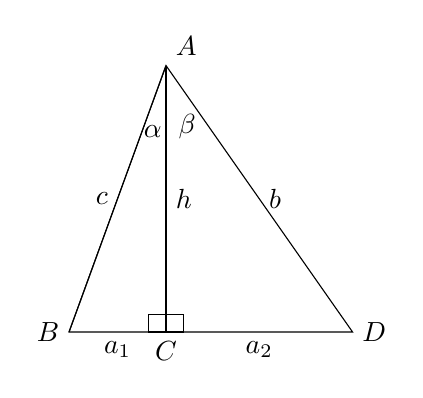
\begin{tikzpicture}[scale=.9]
\coordinate (B) at (0,0);
\node[left] at (B) {$B$};
\coordinate (D) at (4,0);
\node[right] at (D) {$D$};
\draw (B) -- +(70:4) coordinate (A);
\node[above right] at (A) {$A$};
\draw (A) -- node[left] {$c$} (B) -- (D) -- node[right] {$b$} cycle;

\draw (A) -- node[right] {$h$} (A|-B) coordinate (C);
\node[below] at (C) {$C$};
\node[below left,xshift=2pt,yshift=-18pt] at (A) {$\alpha$};
\node[below right,xshift=1pt,yshift=-14pt] at (A) {$\beta$};
\draw[rotate=90] (C) rectangle +(7pt,7pt);
\draw (C) rectangle +(7pt,7pt);
\path (B) -- node[below] {$a_1$} (C) -- node[below] {$a_2$} (D);
\end{tikzpicture}
%\includegraphics[width=0.6\textwidth]{FigA4}

\caption{Calcul de l'aire d'un triangle de deux façons.}\label{f.sin-sum2}
\end{figure}

\enlargethispage{\baselineskip}

La deuxième démonstration utilise le théorème suivant :
\begin{theorem}
Dans un cercle de diamètre 1, la longueur d'une corde qui sous-tend un angle inscrit est égale au sinus de cet angle (fig.~\ref{f.chord-angle}).
\end{theorem}

\begin{figure}[htbp]
\centering
\begin{tikzpicture}[scale=.7]

\coordinate (A) at (0,0);
\coordinate (C) at (3,4);
\coordinate (O) at ($(A)!.5!(C)$);
\vertex{O};
\node[left] at (O) {$O$};
\draw (A) -- (C);
\node[draw,circle through=(A),name path=circle] at (O) {};
\coordinate (B) at ($(O)+(10:2.5)$);
\draw (A) -- (B) -- node[left] {$a$} (C);
\draw[rotate=120] (B) rectangle +(8pt,8pt);
\coordinate (D) at ($(O)+(160:2.5)$);
\draw(C) -- (D) -- (B);
\node[above right,xshift=12pt,yshift=12pt] at (A) {$\alpha$};
\node[right,xshift=16pt,yshift=2pt] at (D) {$\alpha$};
\node[below left] at (A) {$A$};
\node[above right] at (C) {$B$};
\node[right] at (B) {$C$};
\node[left] at (D) {$D$};
\end{tikzpicture}        %\includegraphics[width=0.6\textwidth]{FigA5}

\caption{Tous les angles inscrits sous-tendus par une même corde sont égaux.}\label{f.chord-angle}
\end{figure}

\begin{proof}
Soit $\overline{AB}$ un diamètre et soit $\angle BAC=\alpha$. Soit $D$ un autre point quelconque du cercle. Il forme un triangle 
 $\triangle BDC$ dont l'un des côtés est la corde $\overline{BC}$. Puisque des cordes égales sous-tendent des angles inscrits égaux, $\angle BDC=\alpha$. Dans le triangle rectangle $\triangle ABC$,
\[
\sin \alpha = \frac{\overline{BC}}{\overline{AB}}=\frac{\overline{BC}}{1}=\overline{BC}\,.\qedhere
\]
\end{proof}

\medskip

\noindent \emph{Démonstration 2}. 
Cette démonstration se base sur la figure  de droite de la figure~\ref{f.sin-sum1},  reproduite dans la figure~\ref{f.trig-quad-circle} où le quadrilatère $\overline{ABCD}$ a été inscrit dans un cercle. D'après le théorème~\ref{thm.quad-circum}, un quadrilatère peut être circonscrit par un cercle si et seulement si la somme de chaque paire d'angles opposés est égale à $180^\circ$.
$\angle ADC+\angle ABC=180^\circ$ puisque les deux angles sont des angles droits. D'après le théorème~\ref{thm.interior-angles-of-a-polygon}, la somme des angles intérieurs d'un quadrilatère est de $360^\circ$, donc $\angle DAB+\angle DCB=180^\circ$. 
\begin{figure}[htbp]
\centering
        \begin{tikzpicture}[scale=.8]
\coordinate (A) at (0,0);
\node[left] at (A) {$A$};
\node[right,xshift=6pt,yshift=5pt] at (A) {$\alpha$};
\node[above right,xshift=4pt,yshift=8pt] at (A) {$\beta$};
\coordinate (B) at (3.5,0);
\node[right] at (B) {$B$};
\draw (A) -- +(70:4.5) coordinate (D);
\node[above left] at (D) {$D$};
\path[name path=dc1] (D) -- +(-20:2.5);
\path[name path=bc1] (B) -- +(90:4);
\path[name intersections={of=dc1 and bc1,by={C}}];
\node[above right] at (C) {$C$};
\draw[rotate=90] (B) rectangle +(9pt,9pt);
\draw[rotate=-110] (D) rectangle +(9pt,9pt);
\draw (A) -- (B) -- (C) -- (D) -- cycle;
\draw (A) -- (C);
\draw (D) -- (B);

\coordinate (O) at ($(A)!.5!(C)$);
\node[draw,circle through=(A),name path=circle] at (O) {};
\node[below right,xshift=6pt,yshift=-4pt] at (D) {$\alpha$};
\node[below,xshift=1pt,yshift=-10pt] at (D) {$\gamma$};
\node[below left,xshift=-6pt,yshift=4pt] at (C) {$\delta$};
\node[below,xshift=-4pt,yshift=-6pt] at (C) {$\gamma$};
\node[above left,xshift=-7pt,yshift=4pt] at (B) {$\delta$};
\node[above,xshift=-4pt,yshift=14pt] at (B) {$\beta$};
\end{tikzpicture}
%\includegraphics[width=0.5\textwidth]{FigA6}

\caption{Un quadrilatère circonscrit par un cercle.}\label{f.trig-quad-circle}
\end{figure}

Supposons que le diamètre du cercle soit 1 (sinon, multiplions tout par la longueur du diamètre). Alors les côtés du quadrilatère sont 
\[
\overline{BC}=\sin\alpha,\quad \overline{CD}=\sin\beta,\quad \overline{AB}=\sin\gamma,\quad \overline{DA}=\sin\delta\,.
\]
Les diagonales sont 
\[
\overline{BD}=\sin(\alpha + \beta),\quad \overline{CA}=\sin (\alpha+\gamma)\,.
\]

D'après le théorème de Ptolémée (théorème~\ref{thm.ptolemy}), le produit des diagonales d'un quadrilatère circonscrit à un cercle est égal à la somme des produits des côtés opposés du quadrilatère. Puisque $\angle ADC$ et $\angle ABC$ sont des angles droits, nous avons 
\begin{align*}
\sin (\alpha+\beta)\sin(\alpha+\gamma)&=
\sin \alpha \sin\delta + \sin \beta\sin \gamma,\\
\sin (\alpha+\beta)\sin(90^\circ)&=
\sin \alpha \sin(90^\circ-\beta) + \sin \beta\sin (90^\circ-\alpha),\\
\sin (\alpha+\beta)&=\sin\alpha\cos\beta+\cos\alpha\sin \beta\,. \tag*{\qed}
\end{align*}


%%%%%%%%%%%%%%%%%%%%%%%%%%%%%%%%%%%%%%%%%%%%%%%%%%%%%%%%%%%

\subsection{Le cosinus d'un angle triple}\label{s.cosine}

\begin{theorem}\label{thm.triple-angle}
\[
\cos 3\alpha=4\cos^3\alpha -3\cos\alpha\,.
\]
\end{theorem}
\begin{proof}
La démonstration utilise les formules du théorème~\ref{thm.sum-of-trig} et la formule 
 $\sin^2\alpha+\cos^2\alpha=1$:
\begin{align*}
\cos 3\alpha &= \cos (2\alpha +\alpha)\\
&= \cos 2\alpha\cos\alpha - \sin 2\alpha\sin\alpha\\
&= (\cos^2\alpha -\sin^2\alpha)\cos\alpha - (2\sin\alpha\cos\alpha)\sin\alpha\\
&=\cos^3\alpha - \cos\alpha\sin^2\alpha -2\sin^2\alpha\cos\alpha\\
&=\cos^3\alpha - \cos\alpha +\cos^3\alpha -2\cos\alpha+2\cos^3\alpha\\
&=4\cos^3\alpha -3\cos\alpha\,.\qedhere
\end{align*}
\end{proof}

%%%%%%%%%%%%%%%%%%%%%%%%%%%%%%%%%%%%%%%%%%%%%%%%%%%%%%%%%%%

\subsection{Le sinus et le cosinus d'un demi-angle}\label{s.sine-cosine-half}

\begin{theorem}\label{thm.sine-cosine-half}
Si $\alpha$ est un angle dans un triangle, alors \footnote{La formule générale est plus complexe car les racines carrées peuvent être positives ou négatives selon le quadrant dans lequel se trouve $\alpha/2$. 
Pour un triangle, $0\!<\!\alpha\!<\!180^\circ$, donc $0\!<\!\alpha/2\!<\!90^\circ$ est dans le premier quadrant et le sinus et le cosinus sont tous deux positifs.}
\begin{align*}
\cos \left(\frac{\alpha}{2}\right)&=\sqrt{\frac{1+\cos\alpha}{2}},\\
\sin\left(\frac{\alpha}{2}\right)&=\sqrt{\frac{1-\cos\alpha}{2}}\,.
\end{align*}
\end{theorem}

\begin{proof}
La démonstration utilise les formules du théorème~\ref{thm.sum-of-trig} et la formule $\sin^2\alpha+\cos^2\alpha=1$:
\begin{align*}
\cos \alpha&=\cos \left(2\cdot \frac{\alpha}{2}\right)=\cos \left(\frac{\alpha}{2}\right)\cos\left(\frac{\alpha}{2}\right)-\sin \left(\frac{\alpha}{2}\right)\sin\left(\frac{\alpha}{2}\right)\\
&=2\cos^2 \left(\frac{\alpha}{2}\right)-1\,,\\
\cos \left(\frac{\alpha}{2}\right)&=\sqrt{\frac{1+\cos\alpha}{2}}\,,\\
\sin^2\left(\frac{\alpha}{2}\right)&= 1-\cos^2\left(\frac{\alpha}{2}\right)=1-\frac{1+\cos\alpha}{2}\,,\\
\sin \left(\frac{\alpha}{2}\right)&=\sqrt{\frac{1-\cos\alpha}{2}}\,.\qedhere
\end{align*}
\end{proof}

%%%%%%%%%%%%%%%%%%%%%%%%%%%%%%%%%%%%%%%%%%%%%%%%%%%%%%%%%%%

\subsection{La loi des cosinus}

\begin{theorem}[loi des cosinus]
Dans un triangle $\triangle ABC$ dont les côtés sont $a,b,c$ (fig.~\ref{f.law-cosines2}),\label{thm.law-of-cosines}
\[
c^2=a^2+b^2-2ab\cos \angle ACB\,.
\]
\end{theorem}

\medskip

\noindent \emph{Démonstration 1}.
Traçons la hauteur issue de $C$ et utilisons la définition du cosinus et le théorème de Pythagore :
\begin{subequations}
\begin{align}
c&= x+(c-x)=a\cos \beta + b\cos \alpha\,,\\
c^2&=ac\cos \beta + bc\cos \alpha\,.\label{eq.lc1}
\end{align}
\end{subequations}
De la même manière, traçons  les hauteurs issues de $A$ et de $B$ pour obtenir 
\begin{subequations}
\begin{align}
a^2&=ca\cos \beta + ba\cos \gamma\,,\label{eq.lc2}\\
b^2&=cb\cos \alpha + ab\cos \gamma\,.\label{eq.lc3}
\end{align}
\end{subequations}

En additionnant les équations~\ref{eq.lc2} et \ref{eq.lc3} et en soustrayant l'équation~\ref{eq.lc1}, on obtient 
\begin{align*}
a^2+b^2-c^2&=ca\cos \beta + ba\cos \gamma\\
&\;\; +\,cb\cos \alpha + ab\cos \gamma \\
&\;\; -\,ac\cos \beta - bc\cos \alpha\\
&=2ab\cos \gamma\,,\\
c^2&=a^2+b^2-2ab\cos \gamma\,.\tag*{\qed}
\end{align*}


\begin{figure}[htbp]
\centering
        \begin{tikzpicture}[scale=.65]
  \coordinate[label = left:$A$] (A) at (0,0);
  \coordinate[label = right:$B$] (B) at (6,0);
  \draw (A) -- (40:5) coordinate (C) node[above] {$C$};
  \draw (A) -- (B) -- node[right] {$a$} (C) -- node[left,yshift=4pt,xshift=-2pt] {$b$} cycle;
\node[below,xshift=-4pt,yshift=-6pt] at (C) {$\gamma$};
\node[above right,xshift=8pt] at (A) {$\alpha$};
\node[above left,xshift=-8pt] at (B) {$\beta$};
\coordinate (D) at (A-|C);
\draw (C) -- (D);  
\draw (D) rectangle +(10pt,10pt);
\draw[<->] (0,-.5) -- node[fill=white] {$c$} (6,-0.5);
\draw[<->] (0,-1) -- node[fill=white] {$c-x$} ($(D)+(0,-1)$);
\draw[<->] ($(D)+(0,-1)$) -- node[fill=white] {$x$} (6,-1);
\end{tikzpicture}
%\includegraphics[width=0.6\textwidth]{FigA7}
     
\caption{Première démonstration de la loi des cosinus.}\label{f.law-cosines2}
\end{figure}



\noindent \emph{Démonstration 2}.
La deuxième démonstration utilise le théorème de Ptolémée  (théorème~\ref{thm.ptolemy}).\footnote{La section~\ref{a.ptolemy} utilise la loi des cosinus pour démontrer le théorème de Ptolémée ! La première démonstration de la loi des cosinus permet d'éviter ce raisonnement circulaire. De plus, il existe des démonstrations du théorème de Ptolémée qui n'utilisent pas la loi des cosinus.}

Le triangle $\triangle ABC$ peut être circonscrit par un cercle. 
Construisons un autre triangle $\triangle ABC'$ isométrique à $\triangle ABC$ et inscrit dans le même cercle (fig.~\ref{f.law-cosines3}). Pour cela, on construit en $B$ un angle avec $\overline{AB}$ égal à $\angle CAB$. Il coupe le cercle en $C'$. Puis on construit la droite $\overline{C'A}$.
Puisque les angles sous-tendus par la même corde sont égaux, $\angle AC'B =\angle BCA$, il en est de même pour $\angle CBA=\angle C'AB$ et donc $\triangle ABC'\cong \triangle BAC$ (deux angles et un côté égaux) avec le côté commun $\overline{AB}$.

Traçons les perpendiculaires à $\overline{AB}$ de $C$ à $D$ et de $C'$ à $D'$ de sorte que $x=a\cos \beta$. D'après le théorème de Ptolémée pour le quadrilatère $\overline{ABCC'}$,
\begin{align*}
b^2&=a^2+c(c-2x)\\
&= a^2 + c(c-2a\cos\beta)\\
&=a^2+c^2-2ac\cos\beta\,.\tag*{\qed}
\end{align*}


\begin{figure}[htbp]
\centering
        \begin{tikzpicture}[scale=.8]
\coordinate (origin) at (0,0);
\coordinate (A) at (-3,-1.5);
\coordinate (B) at (3,-1.5);
\node[draw,circle through=(A),name path=circle] at (origin) {};
\node[left] at (A) {$A$};
\node[right] at (B) {$B$};
\path[name path=b1] (A) -- +(40:7cm);
\path[name path=b2] (B) -- +(140:7cm);
\path [name intersections={of=circle and b1,by={C}}];
\node[above] at (C) {$C$};
\path [name intersections={of=circle and b2,by={Cp}}];
\node[above] at (Cp) {$C'$};
\draw (A) -- node[below] {$c$} (B) -- node[right] {$a$} (C) -- node[left,yshift=4pt,xshift=-2pt] {$b$} cycle;
\draw (A) -- (B) -- node[right,yshift=4pt,xshift=2pt] {$b$}(Cp) -- node[left] {$a$} cycle;
\draw (C) -- node[above] {$c-2x$} (Cp);
\coordinate (D) at (C|-B);
\coordinate (Dp) at (Cp|-B);
\draw (C) -- (D);
\draw[rotate=90] (D) rectangle +(8pt,8pt);
\draw (Cp) -- (Dp);
\draw (Dp) rectangle +(8pt,8pt);
\draw[<->] ($(A)+(0,-.8)$) -- node[fill=white] {$x$} ($(Dp)+(0,-.8)$);
\draw[<->] ($(Dp)+(0,-.8)$) -- node[fill=white] {$c-2x$} ($(D)+(0,-.8)$);
\draw[<->] ($(D)+(0,-.8)$) -- node[fill=white] {$x$} ($(B)+(0,-.8)$);
\node[below] at (D) {$D$};
\node[below] at (Dp) {$D'$};
\node[above right,xshift=8pt,yshift=6pt] at (B) {$\beta$};
\draw ($(B)+(-.8,0)$) arc (180:104:.8);
\draw[->] ($(B)+(.4,.5)$) -- +(190:1.12);

\node[above left,xshift=-8pt,yshift=6pt] at (A) {$\beta$};
\draw ($(A)+(.8,0)$) arc (0:76:.8);
\draw[->] ($(A)+(-.4,.5)$) -- +(-10:1.12);
\end{tikzpicture}
%\includegraphics[width=0.8\textwidth]{FigA8}

\caption{Deuxième démonstration  de la loi des cosinus.}\label{f.law-cosines3}
\end{figure}                       

%%%%%%%%%%%%%%%%%%%%%%%%%%%%%%%%%%%%%%%%%%%%%%%%%%%%%%%%%%%



\subsection{La tangente de la somme de deux angles}\label{s.tangent-sum}


\begin{theorem}\label{thm.tangent-sum}
\[
\tan (\alpha+\beta) =\frac{\tan\alpha+\tan\beta}{1-\tan\alpha\tan\beta}\,.
\]
\end{theorem}

\begin{proof}
\begin{align*}
\tan (\alpha+\beta) &= \frac{\sin(\alpha+\beta)}{\cos(\alpha+\beta)}\\
&=\frac{\sin\alpha\cos\beta+\cos\alpha\sin\beta}{\cos\alpha\cos\beta-\sin\alpha\sin\beta}\\
&=\frac{\sin\alpha+\cos\alpha\tan\beta}{\cos\alpha-\sin\alpha\tan\beta}\\
&=\frac{\tan\alpha+\tan\beta}{1-\tan\alpha\tan\beta}\,.\qedhere
\end{align*}
\end{proof}

%%%%%%%%%%%%%%%%%%%%%%%%%%%%%%%%%%%%%%%%%%%%%%%%%%%%%%%%%%%

\subsection{La tangente d'un demi-angle}\label{s.tangent-half}

\begin{theorem}\label{thm.tangent-half}
\[
\tan\left(\frac{\alpha}{2}\right) = \frac{-1\pm\sqrt{1+\tan^2\alpha}}{\tan\alpha}\,.
\]
\end{theorem}
\begin{proof}
On obtient et on résout une équation du second degré en 
$\displaystyle\tan\left(\displaystyle\frac{\alpha}{2}\right)$:
\begin{align*}
&\tan \alpha=\displaystyle\frac{
  \tan\left(\displaystyle\frac{\alpha}{2}\right)+
  \tan\left(\displaystyle\frac{\alpha}{2}\right)
  }{
  1-\tan\left(\displaystyle\frac{\alpha}{2}\right)
    \tan\left(\displaystyle\frac{\alpha}{2}\right)
  },\\
&\tan\alpha \tan^2  \left(\displaystyle\frac{\alpha}{2}\right) + 2 \tan \left(\displaystyle\frac{\alpha}{2}\right) -\tan\alpha =0,\\
&\tan\left(\displaystyle\frac{\alpha}{2}\right) = \displaystyle\frac{-1\pm\sqrt{1+\tan^2\alpha}}{\tan\alpha}\,.\qedhere
\end{align*}
\end{proof}

%%%%%%%%%%%%%%%%%%%%%%%%%%%%%%%%%%%%%%%%%%%%%%%%%%%%%%%%%%%


\subsection{Le produit de trois tangentes}\label{s.tangent-three}

\begin{theorem}\label{thm.tangent3}
Si $\alpha+\beta+\gamma=180^\circ$, alors
\[
\tan\alpha+\tan\beta+\tan\gamma = \tan\alpha\tan\beta\tan\gamma\,.
\]
\end{theorem}

\begin{proof}
\begin{align*}
\tan\gamma &= \tan (180^\circ-(\alpha+\beta))\\
&= -\tan (\alpha+\beta)\\
&= -\frac{\tan\alpha+\tan\beta}{1-\tan\alpha\tan\beta}\,,\\
\tan\alpha\tan\beta\tan\gamma &=\tan\alpha+\tan\beta+\tan\gamma\,.\qedhere
\end{align*}

\end{proof}

%%%%%%%%%%%%%%%%%%%%%%%%%%%%%%%%%%%%%%%%%%%%%%%%%%%%%%%%%%%



\subsection{La limite de $\frac{\sin\alpha}{\alpha}$}\label{s.sin-over-x}

En examinant les polygones réguliers inscrits dans un cercle unité  (fig.~\ref{fig.regular-polygons}), on constate que plus un polygone a de côtés, plus son périmètre est proche de la circonférence du cercle. 


\begin{figure}[htbp]
\centering
        \begin{tikzpicture}[scale=.7]
\coordinate (o1) at (0,0);
\coordinate (a1) at (1.8,0);
\node[draw, name path = circle] at (o1)
    [circle through = (a1)] {};
\foreach \node/\angle in {a2/120,a3/240} {
  \coordinate (\node) at (\angle:1.8);
}
\draw (a1) -- (a2) -- (a3) -- cycle;
\begin{scope}[xshift=5cm]
\coordinate (o2) at (0,0);
\coordinate (b1) at (1.8,0);
\node[draw, name path = circle] at (o2)
    [circle through = (b1)] {};
\foreach \node/\angle in
  {b2/45,b3/90,b4/135,b5/180,b6/-135,b7/-90,b8/-45} {
  \coordinate (\node) at (\angle:1.8);
}
\draw (b1) -- (b2) -- (b3) -- (b4) -- (b5) -- (b6) -- (b7) -- (b8) -- cycle;
\end{scope}
\begin{scope}[xshift=10cm]
\coordinate (o3) at (0,0);
\coordinate (c1) at (1.8,0);
\node[draw, name path = circle] at (o3)
    [circle through = (c1)] {};
\foreach \node/\angle in
  {c2/22.5,c3/45,c4/67.5,c5/90,c6/112.5,c7/135,
   c8/157.5,c9/180,c16/-22.5,c15/-45,c14/-67.5,
   c13/-90,c12/-112.5,c11/-135,c10/-157.5} {
  \coordinate (\node) at (\angle:1.8);
}
\draw (c1) -- (c2) -- (c3) -- (c4) -- (c5) -- (c6) --
  (c7) -- (c8) -- (c9) -- (c10) -- (c11) -- (c12) -- (c13) --
  (c14) -- (c15) -- (c16) -- cycle;
\end{scope}
\end{tikzpicture}
%\includegraphics[width=\textwidth]{FigA9}

\caption{Polygones réguliers à 3, 8 et 16 côtés inscrits dans un cercle.}\label{fig.regular-polygons}
\end{figure}

La circonférence du cercle divisée par le nombre de côtés est la longueur d'un arc dont les extrémités sont les mêmes que celles du côté correspondant. Comme le rapport entre la circonférence du cercle et le périmètre d'un polygone inscrit se rapproche de 1 lorsque le nombre de côtés augmente, il en va de même pour le rapport entre la longueur d'un arc et la corde correspondante. Ceci est illustré par les exemples numériques suivants :

\enlargethispage{\baselineskip}
\vspace{-1ex}

\[
\begin{array}{r@{\hspace{10pt}}r@{\hspace{10pt}}r@{\hspace{10pt}}r}
\hline
\textrm{angle} & \textrm{longueur de l'arc} & \textrm{longueur de la corde} & \textrm{rapport}\\
\hline
80 & \mbox{1,396} & \mbox{1,286}  & \mbox{1,090}\\
60 & \mbox{1,047} & \mbox{1,000}  & \mbox{1,047}\\
40 & \mbox{0,698} & \mbox{0,684} & \mbox{1,006}\\
5  & \mbox{0,087} & \mbox{0,087} &\mbox{1,000} \\\hline
\end{array}
\]

Puisque $a=b=1$, la longueur de la corde $c$ sous-tendant $\alpha$ peut être calculée à partir de la loi des cosinus 
 (fig.~\ref{fig.length-of-a-chord}):
\begin{align*}
c^2&=a^2+b^2-2ab\cos \alpha\,,\\
c&=\sqrt{2-2\cos \alpha}\,.\\
%\lim_{\alpha\rightarrow 0} c&= \sqrt{2-2\cdot 1}=0\,.
\end{align*}


\begin{figure}[htbp]
\centering
        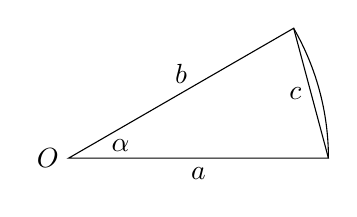
\begin{tikzpicture}[scale=1.1]
  \coordinate  (A) at (3,0);
  \coordinate[label = left:$O$] (O) at (0,0);
  \vertex{O};
  \draw (A) arc(0:30:3) coordinate (B);
  \draw (A) -- node[below] {$a$} (O) -- node[above] {$b$} (B) -- node[left] {$c$} cycle;
  \node[above right,xshift=12pt,yshift=-1pt] at (O) {$\alpha$};
\end{tikzpicture}
%\includegraphics[width=0.6\textwidth]{FigA10}

\caption{La longueur d'une corde correspondant à un arc d'angle $\alpha$.}\label{fig.length-of-a-chord}
\end{figure}


\begin{theorem}\label{thm.limit-sine-over}
\[
\lim_{\alpha\rightarrow 0}\frac{\sin\alpha}{\alpha}=1\,.
\]
\end{theorem}

\begin{proof} En se référant\footnote{N.D.T. On peut remarquer pour $0<\alpha<\pi/2$ que $\sin \alpha \leq \alpha\leq \tan \alpha$ implique $\cos \alpha \leq \tfrac{\sin \alpha}{\alpha} \leq 1$, ce qui donne la limite quand $\alpha \to 0$.} à la figure~\ref{fig.ratio-of-sine-to-x},
\[
\lim_{\alpha \rightarrow 0} \frac{\sin \alpha}{\alpha} = \lim_{\alpha \rightarrow 0} \frac{2\sin \alpha}{2\alpha}\,.
\]
C'est le rapport entre la longueur de la corde $\overline{PQ}$ et la longueur de l'arc $\widehat{PQ}$.
Mais nous avons vu que ce rapport converge vers $1$ lorsque l'angle sous-tendu $2\alpha$ tend vers $0$. Donc 
\[
\lim_{\alpha \rightarrow 0} \frac{\sin \alpha}{\alpha} = 1\,.\qedhere
\]
\end{proof}


\begin{figure}[htbp]
\centering
       \begin{tikzpicture}[scale=.9]
  \draw[thin] (-2,0) -- (2,0);
  \draw[thin] (0,-2) -- (0,2);
  \coordinate[label = above left:$A$]  (A) at (-2,0);
  \coordinate[label = above right:$B$] (B) at (2,0);
  \coordinate[label = above left:$O$] (O) at (0,0);
\vertex{O};
  \node[above right,xshift=6pt] at (O) {$\alpha$} 
    node[below right,xshift=6pt] {$\alpha$};
  \coordinate (P) at (40:2);
  \node[above right] at (P) {$P$};
  \coordinate (Q) at (-40:2);
  \node[draw, name path = circle] at (O)
    [circle through = (A)] {};
  \draw (B)
    arc[start angle=0,end angle=40,radius=2cm];
  \draw (B)
    arc[start angle=0,end angle=-40,radius=2cm];
  \node at (2.1,.8) {$\alpha$};
  \node at (2.1,-.8) {$\alpha$};
  \draw[<->] (P) -- node[fill=white,xshift=-4pt] {$\sin \alpha$}
    (P |- O) coordinate (D);
  \draw[<->] (D) -- node[fill=white,xshift=-4pt] {$\sin \alpha$} (Q);
  \node[below right] at (Q) {$Q$};
  \draw (Q) -- node[below] {$1$} (O) -- node[above] {$1$} (P);
\end{tikzpicture} %\includegraphics[width=0.7\textwidth]{FigA11}

\caption{Rapport entre $\sin \alpha$ et $\alpha$.}\label{fig.ratio-of-sine-to-x}
\end{figure}

%%%%%%%%%%%%%%%%%%%%%%%%%%%%%%%%%%%%%%%%%%%%%%%%%%%%%%%%%%%


\section{Les théorèmes de la bissectrice }\label{a.bisector}


\begin{theorem}\label{thm.angle-bisector}
Dans $\triangle ABC$, la bissectrice de $\angle BAC$ coupe $\overline{BC}$ en $D$  (fig.~\ref{f.angle-bisector}) avec
\[
\frac {\overline{BD}}{\overline{CD}}=\frac {\overline{AB}}{\overline{AC}}\,.
\]
\end{theorem}

\begin{figure}[htbp]
\centering
        \begin{tikzpicture}[scale=.8]
% Draw base and path two lines at known angles
\draw (0,0) coordinate (b) node[left] {$B$} -- (8,0) coordinate (c) node[right] {$C$};
\path[name path=ba] (b) -- +(50:4.5);
\path[name path=ca] (c) -- +(150:7);
% Get their intersection and draw lines between vertices
\path[name intersections={of=ba and ca,by=a}];
\node[above] at (a) {$A$};
\draw (a) -- (c) -- (b) -- (a);
\path[name path=bc] (b) -- (c);
\path[name path=bisector] (a) -- +(-80:4);
\path[name intersections={of= bc and bisector,by=d}];
\node[below] at (d) {$D$};
\draw (a) -- (d);
\node[below left,xshift=2pt,yshift=-8pt] at (a) {$\alpha$};
\node[below right,xshift=2pt,yshift=-8pt] at (a) {$\alpha$};
\draw (a) -- node[left] {$h$} (a |- b);
\draw (a|-b) rectangle +(7pt,7pt);
\end{tikzpicture}
%\includegraphics[width=0.8\textwidth]{FigA12}

\caption{Le théorème de la bissectrice de l'angle interne.}\label{f.angle-bisector}
\end{figure}
\begin{proof}
Nous démontrons le théorème en calculant les aires de deux triangles en utilisant d'une part  la base et la hauteur (équation~\ref{eq.area-from-base}), d'autre part la base, l'angle et le côté (équation~\ref{eq.area-from-sine}):
\begin{align*}
\triangle ABD&=\frac{1}{2}\overline{BD}h=\frac{1}{2}\overline{AB}\,\overline{AD}\sin \alpha\,,\\
\frac{\overline{BD}}{\overline{AB}}&=\frac{\overline{AD}\sin \alpha}{h}\,,\\
\triangle ACD&=\frac{1}{2}\overline{CD}h=\frac{1}{2}\overline{AC}\,\overline{AD}\sin \alpha\,,\\
\frac{\overline{CD}}{\overline{AC}}&=\frac{\overline{AD}\sin \alpha}{h}\,,\\
\frac{\overline{BD}}{\overline{CD}}&=\frac{\overline{AB}}{\overline{AC}}\,.\qedhere
\end{align*}
\end{proof}

Il existe également un théorème de la bissectrice externe :
\begin{theorem}\label{thm.external-angle-bisector}
Dans $\triangle ABC$, soit $\overline{AE}$ la bissectrice de l'angle supplémentaire de l'angle $\triangle BAC$ (fig.~\ref{f.angle-bisector-external}) et soit $E$ l'intersection de la bissectrice et de $\overline{BC}$. Alors 
\[
\frac {\overline{BE}}{\overline{CE}}=\frac {\overline{AB}}{\overline{AC}}\,.
\]
\end{theorem}

\begin{figure}[htbp]
\centering
        \begin{tikzpicture}[scale=1]
% Draw base and path two lines at known angles
\draw (0,0) coordinate (b) node[below] {$B$} -- (6,0) coordinate (c) node[right] {$C$};
\path[name path=ba] (b) -- +(70:2.5);
\draw[name path=ca] (c) -- +(160:7);
% Get their intersection and draw lines between vertices
\path[name intersections={of=ba and ca,by=a}];
\node[above] at (a) {$A$};
\draw (a) -- (c) -- (b) -- (a);
\path[name path=bc] (b) -- (c);
\node[left,xshift=-10pt,yshift=-2pt] at (a) {$\alpha$};
\node[below,xshift=-12pt,yshift=-8pt] at (a) {$\alpha$};
\path[name path=ext-bisector] (a) -- +(-155:4.7);
\draw[name path=ext-bc] (c) -- ($(c)!1.6!(b)$);
\path[name intersections={of=ext-bc and ext-bisector,by=e}];
\draw (a) -- (e) node[below] {$E$};
\coordinate (d) at (a |- b);
\draw (a) -- node[right] {$h$} (d);
\draw (d) rectangle +(6pt,6pt);
\end{tikzpicture}
%\includegraphics[width=\textwidth]{FigA13}

\caption{Le théorème de la bissectrice de l'angle externe.}\label{f.angle-bisector-external}
\end{figure}



\begin{proof} On a $\angle EAC=180^\circ-\alpha$.
\begin{align*}
\triangle ABE&=\frac{1}{2}\overline{BE}h=\frac{1}{2}\overline{AE}\,\overline{AB}\sin \alpha\,,\\
\triangle ACE&=\frac{1}{2}\overline{CE}h=\frac{1}{2}\overline{AE}\,\overline{AC}\sin (180^\circ-\alpha)=\frac{1}{2}\overline{AE}\,\overline{AC}\sin \alpha\,,\\
\frac{\overline{BE}}{\overline{AB}}&=\frac{\overline{AE}\sin \alpha}{h}=\frac{\overline{CE}}{\overline{AC}}\,,\\
\frac{\overline{BE}}{\overline{CE}}&=\frac{\overline{AB}}{\overline{AC}}\,. \qedhere
\end{align*}
\end{proof}

%%%%%%%%%%%%%%%%%%%%%%%%%%%%%%%%%%%%%%%%%%%%%%%%%%%%%%%%%%%

\section{Le théorème de Ptolémée}\label{a.ptolemy}


%%%%%%%%%%%%%%%%%%%%%%%%%%%%%%%%%%%%%%%%%%%%%%%%%%%%%%%%%%%

\subsection{Un trapèze circonscrit par un cercle}\label{s.circumscribed}

Avant de donner la démonstration du théorème de Ptolémée, nous démontrons des théorèmes sur les quadrilatères et les trapèzes.

\begin{theorem}\label{thm.quad-circum}
Un quadrilatère peut être circonscrit par un cercle si et seulement si les angles opposés sont supplémentaires (somme égale à $180^\circ$).
\end{theorem}

Les manuels de géométrie donnent la démonstration simple du sens direct, mais il est difficile de trouver une démonstration de la réciproque. C'est pourquoi nous donnons ici les deux démonstrations.

\noindent \emph{Démonstration (sens direct)}. 
Un angle inscrit est égal à la moitié de l'arc qui le sous-tend. Ainsi, $\angle DAB$ est la moitié de l'arc $\widehat{DCB}$ et $\angle DCB$ est la moitié de l'arc $\widehat{DAB}$ (fig.~\ref{f.trap-1}). Ces deux arcs forment la totalité de la circonférence du cercle, leur somme est donc de $360^\circ$. Par conséquent, $\angle DAB + \angle DCB = \frac{1}{2} \cdot 360^\circ = 180^\circ$, et de même $\angle ADC + \angle ABC = 180^\circ$.\qed



\vspace{0.4cm}

\begin{minipage}{0.4\textwidth}
\centering 
\begin{tikzpicture}[scale=.55]
\coordinate (origin) at (0,0);
\coordinate (A) at (1,3);
\node[draw,circle through=(A),name path=circle] at (origin) {};
\node[above right] at (A) {$A$};
\path[name path=b] (A) -- (-50:4.5cm);
\path[name path=c] (A) -- (-120:4.5cm);
\path[name path=d] (A) -- (150:4.5cm);
\path [name intersections={of=circle and b,by={b1,B}}];
\node[right] at (B) {$B$};
\path [name intersections={of=circle and c,by={c1,C}}];
\node[below left] at (C) {$C$};
\path [name intersections={of=circle and d,by={d1,D}}];
\node[above left] at (D) {$D$};
\draw (A) -- (B) -- (C) -- (D) -- cycle;
\end{tikzpicture}
%\includegraphics[width=0.9\textwidth]{FigA14a}
         \captionof{figure}{Un quadrilatère circonscrit par un cercle.}\label{f.trap-1}
         
     \end{minipage}
     \hspace{3em}
     \begin{minipage}{0.4\textwidth}
\centering         \begin{tikzpicture}[scale=.55]
\coordinate (origin) at (0,0);
\coordinate (A) at (1,3);
\node[draw,circle through=(A),name path=circle] at (origin) {};
\node[above right] at (A) {$A$};
\path[name path=b] (A) -- (-50:4cm);
\path[name path=c] (A) -- (-120:4cm);
\path[name path=d] (A) -- (150:4cm);
\path [name intersections={of=circle and b,by={b1,B}}];
\node[right] at (B) {$B$};
\path [name intersections={of=circle and c,by={c1,C}}];
\node[below left] at (C) {$C$};
\path [name intersections={of=circle and d,by={d2,D}}];
\node[above left] at (D) {$D$};
\coordinate (Cp) at ($(C)!.2!(D)$);
\draw (A) -- (B) -- (Cp) -- (D) -- cycle;
\node[left,xshift=1pt,yshift=2pt] at (Cp) {$C'$};
\draw (D) -- (B) -- (C) -- (Cp);
\end{tikzpicture}
%\includegraphics[width=0.9\textwidth]{FigA14b}
         \captionof{figure}{Le quatrième sommet doit être sur la circonférence.}\label{f.trap-2}
     \end{minipage}

\vspace{0.4cm}


\noindent \emph{Démonstration de la réciproque}. 
Tout triangle peut être circonscrit par un cercle. On circonscrit $\triangle DAB$ par un cercle et on suppose que $C'$ est un point tel que $\angle DAB + \angle DC'B = 180^\circ$, mais $C'$ n'est pas sur la circonférence du cercle. Sans perte de généralité, supposons que $C'$ soit situé à l'intérieur du cercle  (fig.~\ref{f.trap-2}).

Construisons une demi-droite qui prolonge $\overline{DC'}$. Soit $C$ son intersection avec le cercle. $\overline{ABCD}$ est circonscrit par un cercle, donc 
\begin{align*}
\angle DAB + \angle DCB &=  180^\circ = \angle DAB + \angle DC'B\,,\\
\angle DCB &= \angle DC'B\,,
\end{align*}
ce qui est impossible si $C$ est sur le cercle et $C'$ est à l'intérieur du cercle. \qed

\begin{theorem}\label{thm.isoceles-trapezoid}
Les angles opposés d'un trapèze isocèle sont supplémentaires.
\end{theorem}
\begin{proof}
Construisons le segment $\overline{AB'}$ parallèle à $\overline{CD}$ (fig.~\ref{f.trap-3}). $\overline{AB'CD}$ est un parallélogramme et  $\triangle ABB'$ est un triangle isocèle, donc $\angle C= \angle AB'B = \angle ABB' = \angle B$. De même, $\angle A = \angle D$. Puisque la somme des angles internes de tout quadrilatère est égale à $360^\circ$,
\begin{align*}
\angle A + \angle B + \angle C + \angle D &= 360^\circ\,,\\
2\angle A + 2 \angle C &= 360^\circ\,,\\
\angle A +  \angle C &= 180^\circ\,,
\end{align*}
et de même $\angle B +  \angle D = 180^\circ$.
\end{proof}

\begin{theorem}
Un trapèze isocèle peut être circonscrit par un cercle.
\end{theorem}
La démonstration est immédiate d'après les théorèmes~\ref{thm.quad-circum} et  \ref{thm.isoceles-trapezoid}.

\begin{figure}[htbp]
\centering
        \begin{tikzpicture}[scale=.65]
\clip (-4.5,-2) rectangle (4.5,2.8);
\coordinate (origin) at (0,0);
\coordinate (A) at (2.5,1.8);
\node[circle through=(A),name path=circle] at (origin) {};
\node[above right] at (A) {$A$};
\path[name path=b] (A) -- ++(-80:4cm);
\path[name path=d] (A) -- ++(180:6cm);
\path [name intersections={of=circle and b,by={b1,B}}];
\node[below right] at (B) {$B$};
\path [name intersections={of=circle and d,by={d1,D}}];
\node[above left] at (D) {$D$};
\path[name path=c] (D) -- ++(-100:4cm);
\path [name intersections={of=circle and c,by={c1,C}}];
\node[below left] at (C) {$C$};
\draw (A) -- node[right] {$x$} (B);
\draw[name path=bc] (B) -- node[below] {$y$} (C);
\draw (C) -- node[left] {$x$} (D) -- node[above] {$y$} (A);
\path[name path=para] (A) -- ++(-100:4cm);
\path [name intersections={of=para and bc,by={Bp}}];
\node[below left] at (Bp) {$B'$};
\draw (A) -- node[left,xshift=-2pt] {$x$} (Bp);
\end{tikzpicture}
%\includegraphics[width=0.6\textwidth]{FigA15}

\caption{Un trapèze isocèle.}\label{f.trap-3}
\end{figure}

%%%%%%%%%%%%%%%%%%%%%%%%%%%%%%%%%%%%%%%%%%%%%%%%%%%%%%%%%%%
\subsection{Démonstration du théorème de Ptolémée}

\begin{theorem}[Ptolémée] Étant donné un quadrilatère circonscrit par un cercle, la formule suivante met en relation les longueurs des diagonales et les longueurs des côtés  (fig.~\ref{f.trig-ptolemy}):\label{thm.ptolemy}
\[
ef = ac + bd\,.
\]
\end{theorem}

\begin{figure}[htbp]
\centering
        \begin{tikzpicture}[scale=.5]
\coordinate (origin) at (0,0);
\coordinate (A) at (1,3);
\node[draw,circle through=(A),name path=circle] at (origin) {};
\node[above right] at (A) {$A$};
\path[name path=b] (A) -- (-50:4cm);
\path[name path=c] (A) -- (-120:4cm);
\path[name path=d] (A) -- (150:4cm);
\path [name intersections={of=circle and b,by={b1,B}}];
\node[right] at (B) {$B$};
\path [name intersections={of=circle and c,by={C,c2}}];
\node[below left] at (C) {$C$};
\path [name intersections={of=circle and d,by={D,d2}}];
\node[above left] at (D) {$D$};
\draw (A) -- node[right] {$a$} (B) -- node[below,yshift=-10pt] {$b$} (C) -- node[left] {$c$} (D) -- node[above,xshift=2pt,yshift=8pt] {$d$}  cycle;
\draw (A) -- node[right,near start] {$e$} (C);
\draw (B) -- node[left,near end,yshift=-6pt] {$f$} (D);
\end{tikzpicture}
%\includegraphics[width=0.5\textwidth]{FigA16}

\caption{Le théorème de Ptolémée}\label{f.trig-ptolemy}
\end{figure}                       

\begin{proof}
D'après la loi des cosinus pour les quatre triangles  $\triangle ABC$, $\triangle ADC$, $\triangle DAB$ et $\triangle DCB$,
\begin{align*}
e^2 &= a^2 + b^2 - 2ab \cos \angle B,\\
e^2 &= c^2 + d^2 - 2cd \cos \angle D,\\
f^2 &= a^2 + d^2 - 2ad \cos \angle A,\\
f^2 &= b^2 + c^2 - 2bc \cos \angle C\,.
\end{align*}
$\angle C = 180^\circ - \angle A$ et $\angle D = 180^\circ - \angle B$ car ce sont des angles opposés d'un quadrilatère circonscrit par un cercle, donc $\cos \angle D = - \cos \angle B$ et $\cos \angle C = -\cos \angle A$. Éliminons le terme en cosinus des équations ci-dessus pour obtenir 
\begin{align*}
e^2(cd+ab)&=abc^2+abd^2+a^2cd+b^2cd\,,\\
e^2 &= \frac{(ac+bd)(ad+bc)}{(ab+cd)}\,,\\
f^2 &= \frac{(ab+cd)(ac+bd)}{(ad+bc)}\,.
\end{align*}
Multiplions les deux équations et simplifions pour obtenir le théorème de Ptolémée 
\begin{align*}
e^2\cdot f^2 &= (ac+bd)^2\,,\\
ef &= ac+bd\,.\qedhere
\end{align*}
\end{proof}

%%%%%%%%%%%%%%%%%%%%%%%%%%%%%%%%%%%%%%%%%%%%%%%%%%%%%%%%%%%

\section{Le théorème de Ceva}\label{a.ceva}

\begin{theorem}[Ceva]
Pour des segments  qui vont des sommets d'un triangle aux côtés opposés et qui se coupent en un point, les longueurs des segments (fig.~\ref{f.ceva1}) vérifient 
  \label{thm.ceva}
\[
\frac{\overline{AM}}{\overline{MB}}\cdot\frac{\overline{BQ}}{\overline{QS}}\cdot\frac{\overline{SP}}{\overline{PA}} = 1\,.
\]
\end{theorem}

\begin{figure}[htbp]
\centering
        \begin{tikzpicture}[scale=.9]
\path[name path=pq] (-4,0) -- (4,0);
\draw (-2,-2) node[below left] {$A$} coordinate (A) -- (2,-2) node[below right] {$B$} coordinate (B);
\draw[name path=as] (A) -- ++(50:4cm) node[above] {$S$} coordinate (S);
\draw[name path=sb] (S) -- (B);
\path [name intersections={of=pq and as,by={P}}];
\path [name intersections={of=pq and sb,by={Q}}];
\node[above left] at (P) {$P$};
\node[above right] at (Q) {$Q$};
\draw[name path=pb] (P) -- (B);
\draw[name path=qa] (Q) -- (A);
\path [name intersections={of=pb and qa,by={O}}];
\node[right,xshift=2pt] at (O) {$O$};
\coordinate (M) at (0,-2);
\node[below right] at (M) {$M$};
\draw (S) -- (M);
\end{tikzpicture}
%\includegraphics[width=0.5\textwidth]{FigA17}

\caption{Le théorème de Ceva}\label{f.ceva1}
\end{figure}

\begin{proof} Si les hauteurs de deux triangles sont égales, leurs aires sont proportionnelles aux bases. Dans les deux représentations de la figure~\ref{f.ceva2}, les hauteurs des triangles gris sont égales, donc 
\[
\frac{\triangle BQO}{\triangle SQO} = \frac{\overline{BQ}}{\overline{QS}}\;,\quad\quad \frac{\triangle BQA}{\triangle SQA} = \frac{\overline{BQ}}{\overline{QS}}\;.
\]



\begin{figure}[th]
\centering
      \begin{tikzpicture}[scale=.9]
\clip (-2.2,-2.4) rectangle +(10.4,4);
\path[name path=pq] (-4,0) -- (4,0);
\draw (-2,-2) node[below] {$A$} coordinate (A) -- (2,-2) node[below] {$B$} coordinate (B);
\coordinate (M) at (0,-2);
\draw[name path=as] (A) -- ++(50:4cm) node[above] {$S$} coordinate (S);
\draw[name path=sb] (S) -- (B);
\path [name intersections={of=pq and as,by={P}}];
\path [name intersections={of=pq and sb,by={Q}}];
\path[name path=pb] (P) -- (B);
\path[name path=qa] (Q) -- (A);
\path [name intersections={of=pb and qa,by={O}}];
\draw[fill=gray!40] (B) -- (O) -- (Q);
\draw[fill=gray!70] (S) -- (O) -- (Q);
\draw (B) -- (O) -- (A);
\draw (S) -- (O) -- (A);
\draw (A) -- (B) -- (S) -- cycle;
\draw (S) -- (O);
\draw (B) -- (O);
\node[above right] at (Q) {$Q$};
\node[above left] at (O) {$O$};
\path[name path=al1] (O) -- ($(Q)!(O)!(B)$);
\path [name intersections={of=al1 and sb,by={A1}}];
\draw (O) -- (A1);
\draw[rotate=-156] (A1) rectangle +(7pt,7pt);
\begin{scope}[xshift=6cm]
\path[name path=pq] (-4,0) -- (4,0);
\draw (-2,-2) node[below] {$A$} coordinate (A) -- (2,-2) node[below] {$B$} coordinate (B);
\coordinate (M) at (0,-2);
\draw[name path=as] (A) -- ++(50:4cm) node[above] {$S$} coordinate (S);
\draw[name path=sb] (S) -- (B);
\path [name intersections={of=pq and as,by={P}}];
\path [name intersections={of=pq and sb,by={Q}}];
\draw[name path=pb] (P) -- (B);
\draw[name path=qa] (Q) -- (A);
\path [name intersections={of=pb and qa,by={O}}];
\draw (B) -- (O) -- (Q);
\draw (A) -- (Q) -- (B);
\draw[fill=gray!40] (B) -- (Q) -- (A);
\draw[fill=gray!70] (S) -- (Q) -- (A);
\draw (A) -- (B) -- (S) -- cycle;
\draw (S) -- (O);
\draw (B) -- (O);
\node[above right] at (Q) {$Q$};
\node[above left] at (O) {$O$};
\path[name path=al2] (A) -- ($(Q)!(A)!(B)$);
\path [name intersections={of=al2 and sb,by={A2}}];
\draw (A) -- (A2);
\draw[rotate=-156] (A2) rectangle +(7pt,7pt);
\end{scope}
\end{tikzpicture}  %\includegraphics[width=\textwidth]{FigA18}

\caption{Triangles dans le théorème de Ceva.}\label{f.ceva2}
\end{figure}

En soustrayant les surfaces des triangles indiqués, on obtient le rapport entre les aires des triangles gris de la figure~\ref{f.ceva3}:
\[
\frac{\triangle BOA}{\triangle SOA}=\frac{\triangle BQA - \triangle BQO}{\triangle SQA-\triangle SQO} = \frac{\overline{BQ}}{\overline{QS}}\,.
\]

%\newpage

\begin{figure}[htbp]
\centering
        \begin{tikzpicture}[scale=.9]
\path[name path=pq] (-4,0) -- (4,0);
\draw (-2,-2) node[below left] {$A$} coordinate (A) -- (2,-2) node[below right] {$B$} coordinate (B);
\coordinate (M) at (0,-2);
\draw[name path=as] (A) -- ++(50:4cm) node[above] {$S$} coordinate (S);
\draw[name path=sb] (S) -- (B);
\path [name intersections={of=pq and as,by={P}}];
\path [name intersections={of=pq and sb,by={Q}}];
\path[name path=pb] (P) -- (B);
\draw[thick,name path=qa] (Q) -- (A);
\path [name intersections={of=pb and qa,by={O}}];
\draw[fill=gray!50] (B) -- (O) -- (A);
\draw[fill=gray!70] (S) -- (O) -- (A);
\draw (B) -- (O) -- (A);
\draw (S) -- (O) -- (A);
\draw (A) -- (B) -- (S) -- cycle;
\draw (S) -- (O);
\draw (B) -- (O);
\node[above right] at (Q) {$Q$};
\node[right,xshift=2pt] at (O) {$O$};
\end{tikzpicture}
%\includegraphics[width=0.5\textwidth]{FigA19}

\caption{Soustraction d'aires dans le théorème de Ceva.}\label{f.ceva3}
\end{figure}

Cela peut sembler étrange au premier abord. Nous allons donc l'expliquer en utilisant une notation plus simple :
\begin{align*}
 \frac{c}{d} &=\frac{a}{b}\,,\\
 \frac{e}{f} &=\frac{a}{b}\,,\\
c-e &= \frac{ad}{b} - \frac{af}{b}=\frac{a}{b}(d-f)\,,\\
\frac{c-e}{d-f} &= \frac{a}{b}\,.
\end{align*}
De même, nous pouvons démontrer :
\begin{align*}
\frac{\overline{AM}}{\overline{MB}} &= \frac{\triangle AOS}{\triangle BOS}\,,\\
\frac{\overline{SP}}{\overline{PA}} &=\frac{\triangle SOB}{\triangle AOB}\,,
\end{align*}
donc
\[
\frac{\overline{AM}}{\overline{MB}}\frac{\overline{BQ}}{\overline{QS}}\frac{\overline{SP}}{\overline{PA}} = \frac{\triangle AOS}{\triangle BOS}\frac{\triangle BOA}{\triangle SOA}\frac{\triangle SOB}{\triangle AOB}=1\,,
\]
puisque l'ordre des sommets dans un triangle ne fait aucune différence.
\end{proof}

\section{Le théorème de Ménélaüs}\label{a.menelaus}

\begin{theorem}[Ménélaüs]\label{thm.menelaus} 
Soit $\triangle ABC$ un triangle et $\overline{DBQ}$ une droite transversale qui coupe les trois côtés du triangle ou leurs prolongements (fig.~\ref{f.menelaus}). Alors \footnote{Selon la configuration du triangle et de la droite transversale, le résultat de la multiplication peut être plus ou moins un.}
\begin{align}
\displaystyle\frac{\overline{AB}}{\overline{BP}}\cdot
\displaystyle\frac{\overline{PQ}}{\overline{QC}}\cdot
\displaystyle\frac{\overline{CD}}{\overline{AD}}=1\,.\label{eq.menelaus}
\end{align}
\end{theorem}


\begin{figure}[htbp]
\centering
        \begin{tikzpicture}[scale=.6]
\clip (-.8,-.4) rectangle +(11.2,6.5);
\coordinate (D) at (0,0) node[left] {$D$};
\draw (D) -- ++(60:6) coordinate (C) node[left] {$C$};
\coordinate (A) at (60:3);
\node[left] at (A) {$A$};
\draw (A) -- ++(3,0) coordinate (B) -- (C);
\node[below right] at (B) {$B$};
\path[name path=DQ] (D) -- ($(D)!1.7!(B)$);
\path[name path=AP] (A) -- ($(A)!3!(B)$);
% 3*(1+\sqrt[3]{2}) = 6.78
\path[name path=CP] (C) circle (6.78cm);
\path[name intersections={of=CP and AP,by={P}}];
\draw[name path=CP] (C) -- (P);
\path[name intersections={of=CP and DQ,by={Q}}];
\node[above] at (Q) {$Q$};
\node[right] at (P) {$P$};
\draw (D) -- (Q);
\draw (B) -- (P);
\path[dashed,name path=CK] (C) -- ($(C)+(6.5,0)$);
\path[name path=DK] (D) -- ($(D)!2!(Q)$);
\path[name intersections={of=DK and CK,by={K}}];
\draw[dashed] (Q) -- (K) node[right] {$K$} -- (C);
\draw[very thick] (Q) -- (D);
\draw[dashed] (C) -- (K) -- (Q);
\draw (B) -- (P) -- (C);
\end{tikzpicture}
%\includegraphics[width=0.7\textwidth]{FigA20}
\caption{Le théorème de Ménélaüs.}\label{f.menelaus}
\end{figure}

\begin{proof}
Traçons une droite passant par $C$ et parallèle à $\overline{AB}$. Prolongeons $\overline{DQ}$ jusqu'à ce qu'elle coupe la parallèle en $K$. De $\triangle ADB \sim \triangle CDK$, il résulte que 
\begin{equation*}
\displaystyle\frac{\overline{CD}}{\overline{AD}}=\displaystyle\frac{\overline{CK}}{\overline{AB}}\,.
\end{equation*}
De $\triangle  BQP\sim \triangle KQC$, on déduit
\begin{equation*}
\displaystyle\frac{\overline{QC}}{\overline{PQ}}=\displaystyle\frac{\overline{CK}}{\overline{BP}}\,.
\end{equation*}
L'élimination de  $\overline{CK}$ donne 
$\overline{AB}\cdot\overline{CD}\cdot\overline{PQ}=\overline{QC}\cdot\overline{BP}\cdot\overline{AD}$,  qui peut être réarrangé pour obtenir l'équation~\ref{eq.menelaus}.
\end{proof}

%%%%%%%%%%%%%%%%%%%%%%%%%%%%%%%%%%%%%%%%%%%%%%%%%%%%%%%%%%%

\subsection*{Sources}

Cette annexe se base principalement sur \cite{gelfand}. Le théorème de Ceva et le théorème de Ménélaüs peuvent être démontrés l'un à partir de l'autre \cite{silvester}.
